\documentclass[aspectratio=169,11pt]{beamer}

\usepackage{graphicx}
\usepackage{tikz}
\usetikzlibrary{positioning,arrows.meta}
\usepackage{xcolor}
\usepackage{booktabs}
\usepackage{tabularx}
\usepackage{array}
\usepackage{ragged2e}

\definecolor{GEUBlue}{RGB}{20,55,105}
\definecolor{GEULightBlue}{RGB}{238,244,251}
\definecolor{GEUGrey}{RGB}{90,90,90}
\definecolor{GEULightGrey}{RGB}{245,246,248}

\usetheme{default}
\setbeamertemplate{navigation symbols}{}
\setbeamertemplate{blocks}[rounded][shadow=false]
\setbeamercolor{normal text}{fg=black,bg=white}
\setbeamercolor{frametitle}{fg=GEUBlue}
\setbeamercolor{structure}{fg=GEUBlue}
\setbeamercolor{block title}{fg=GEUBlue,bg=GEULightBlue}
\setbeamercolor{block body}{fg=black,bg=GEULightBlue}
\setbeamerfont{frametitle}{size=\Large,series=\bfseries}

% Replace with the actual logo filename
\newcommand{\GEULogo}{graphicera_logo.png}

% Header and footer
\setbeamertemplate{headline}{%
  \begin{tikzpicture}[remember picture,overlay]
    \node[anchor=north east,xshift=-0.30cm,yshift=-0.12cm]
      at (current page.north east)
      {\includegraphics[height=0.62cm]{\GEULogo}};
  \end{tikzpicture}
  \vspace{0.72cm}
}
\setbeamertemplate{frametitle}{%
  \vspace{0.03cm}
  \insertframetitle\par
  \vspace{0.04cm}
  \textcolor{GEUBlue}{\rule{\textwidth}{0.9pt}}
  \vspace{0.03cm}
}
\setbeamertemplate{footline}{%
  \leavevmode
  \hbox{%
  \begin{beamercolorbox}[wd=.82\paperwidth,ht=0.32cm,dp=0.10cm,leftskip=.3cm]{author in head/foot}
    \tiny Department of Computer Science \& Engineering | Graphic Era (Deemed to be University)
  \end{beamercolorbox}%
  \begin{beamercolorbox}[wd=.18\paperwidth,ht=0.32cm,dp=0.10cm,rightskip=.3cm]{date in head/foot}
    \hfill\tiny\insertframenumber/\inserttotalframenumber
  \end{beamercolorbox}}
}

\newcommand{\smallnote}[1]{\vspace{0.08cm}{\scriptsize\color{GEUGrey}#1}}
\newcommand{\placeholder}[1]{\textit{\color{GEUGrey}#1}}

\title{\textbf{Project-Based Learning}\\[2mm]\large Phase-I Evaluation}
\author{\textbf{Project Title}\\Team ID: XXXX}
\institute{Department of Computer Science \& Engineering\\Graphic Era (Deemed to be University), Dehradun}
\date{Academic Session 2026--27}

\begin{document}

% 1
\begin{frame}[plain]
\begin{tikzpicture}[remember picture,overlay]
\draw[GEUBlue,line width=3pt] (current page.north west) -- (current page.north east);
\node[anchor=north east,xshift=-0.45cm,yshift=-0.35cm] at (current page.north east)
{\includegraphics[height=1.0cm]{\GEULogo}};
\node[align=center,text width=.84\paperwidth] at ([yshift=.25cm]current page.center)
{{\color{GEUBlue}\fontsize{26}{30}\selectfont\bfseries PROJECT-BASED LEARNING}\\[3mm]
 {\fontsize{18}{22}\selectfont PHASE-I EVALUATION}\\[7mm]
 {\color{GEUGrey}\Large\bfseries \placeholder{Adaptive Traffic Signal System with Emergency Evacuation Support}}\\[3mm]
 {\color{GEUBlue}\normalsize Team ID: DSCPP-III-2026-T179}};
\node[align=center,anchor=south,yshift=.42cm] at (current page.south)
{\bfseries Department of Computer Science \& Engineering\\
Graphic Era (Deemed to be University), Dehradun\\[-1mm]
\scriptsize Academic Session 2026--27};
\end{tikzpicture}
\end{frame}

% 2
\begin{frame}{Team \& Mentor Details}
\begin{columns}[T,totalwidth=\textwidth]
\column{.48\textwidth}
\begin{block}{Team Information}
\begin{tabular}{@{}ll@{}}
\textbf{Team ID:} & T179\\
\textbf{Semester:} & 3rd\\
\textbf{Section:} & A,H,DS1,DS2\\
\textbf{Domain:} & \placeholder{DSA/C++}
\end{tabular}
\end{block}
\column{.48\textwidth}
\begin{block}{Team Members}
1.\quad \placeholder{Riya Goyal -- 2510013064}\\
2.\quad \placeholder{Divya Smriti -- 2510012531}\\
3.\quad \placeholder{Anushka Verma -- 2510380276}\\
4.\quad \placeholder{Tanishka Soni -- 2510380269}
\end{block}
\end{columns}
\vspace{2mm}
\begin{block}{Mentor}
\placeholder{Mr.Ram Ji Chauhan}
\hfill
\textbf{Interactions completed: 3} 
\end{block}
\end{frame}

% 3
\begin{frame}{Problem Statement \& Motivation}
\begin{block}{Problem Statement}
\placeholder{Traffic congestion is the most common problem at busy road junctions. Traffic signals works independently of the no. of vehicles on road. This leads to unnecessary waiting in traffic jam and become difficult during emergencies. To solve this problem our C++ and DSA based traffic simulation adjust signal timing and provides priority to emergency vehicles.}
\end{block}
\vspace{2mm}
\begin{columns}[T,totalwidth=\textwidth]
\column{.48\textwidth}
\textbf{\color{GEUBlue}Motivation}
\begin{itemize}\itemsep1pt
\item \placeholder{Unnecessary traffic jam}
\item \placeholder{Emergency Vehicles face delays}
\item \placeholder{Less efficient normal systems}
\end{itemize}
\column{.48\textwidth}
\textbf{\color{GEUBlue}Target Users / Stakeholders}
\begin{itemize}\itemsep1pt
\item \placeholder{Emergency services}
\item \placeholder{Pedestrians, Drivers}
\item \placeholder{Less congestion, better traffic flow }
\end{itemize}
\end{columns}
\end{frame}

% 4
\begin{frame}{Objectives}
\textbf{\color{GEUBlue}Project Objectives}
\vspace{2mm}
\begin{enumerate}\itemsep5pt
\item \placeholder{To make traffic management easier at busy roads.}
\item \placeholder{To find a better route during emergency.}
\item \placeholder{To help emergency vehicles move quickly through traffic.}
\item \placeholder{To change traffic signals according traffic situations.}
\item \placeholder{To combine C++ concepts.}
\end{enumerate}
\vfill
\begin{center}
\colorbox{GEULightBlue}{\parbox{.80\textwidth}{\centering
\textbf{Key Objective:} \placeholder{To reduce traffic delays and help emergency vehicles reach there destination on time.}}}
\end{center}
\end{frame}

% 5
\begin{frame}{Proposed Solution}
\begin{columns}[T,totalwidth=\textwidth]
\column{.48\textwidth}
\textbf{\color{GEUBlue}Proposed Approach}
\begin{enumerate}\itemsep1pt
\item \placeholder{Take details of roads, traffic, emergencies}
\item \placeholder{Search shortest road and manage signals for traffic}
\item \placeholder{In emergency, emergency vehicles are given high priority}
\item \placeholder{Store details of road, junction, vehicles and traffic signals}
\item \placeholder{Displays valid route, signal changes}
\end{enumerate}
\column{.48\textwidth}
\textbf{\color{GEUBlue}Key Features}
\begin{itemize}\itemsep3pt
\item \placeholder{Shortest route selection}
\item \placeholder{Traffic based signal control}
\item \placeholder{Emergency vehicle priority}
\item \placeholder{Blocked road handling}
\item \placeholder{Simple traffic handling}
\end{itemize}
\end{columns}
\vfill
\smallnote{Helps in Traffic management during normal situation and emergencies and finds the most suitable and shortest route.}
\end{frame}

% 6
\begin{frame}{Integration of PBL Course Concepts}
\scriptsize
\begin{center}
\renewcommand{\arraystretch}{1.25}
\begin{tabularx}{.96\textwidth}{@{}>{\bfseries}p{3.0cm}X p{2.5cm}@{}}
\toprule
Course & Concepts Applied & Project Module\\
\midrule
Data Structures in C & \placeholder{Graph, Queue, Priority Queue, Searching, Sorting} & \placeholder{Route Management Module}\\
OOPs with C++ & \placeholder{Classes, Objects, Inheritance, Polymorphism, Encapsulation} & \placeholder{Traffic Control Module}\\
\midrule
File Handling & \placeholder{File Creation, Reading, Writing, Data Storage} & \placeholder{Data Management Module}\\
\bottomrule
\end{tabularx}
\end{center}
\vfill
\begin{center}
\colorbox{GEULightBlue}{\parbox{.86\textwidth}{\centering
\textbf{Requirement:} Demonstrate meaningful integration of Data Structures, OOP Concepts and File Handling in \textbf{single} project.}}
\end{center}
\end{frame}

% 7
\begin{frame}{System Architecture / Workflow}
\begin{center}
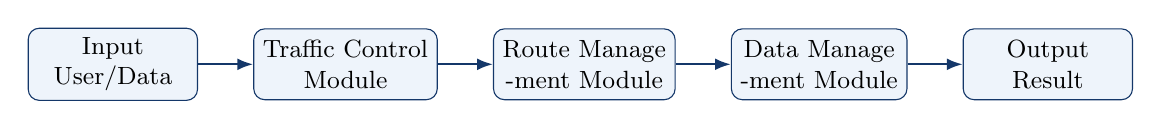
\begin{tikzpicture}[
node distance=7mm,
box/.style={rectangle,rounded corners,draw=GEUBlue,fill=GEULightBlue,
minimum width=2.15cm,minimum height=9mm,align=center,font=\small},
arrow/.style={-{Latex[length=2mm]},thick,draw=GEUBlue}
]
\node[box] (a) {Input\\User/Data};
\node[box,right=of a] (b) {Traffic Control\\Module};
\node[box,right=of b] (c) {Route Manage\\-ment Module};
\node[box,right=of c] (d) {Data Manage\\-ment Module};
\node[box,right=of d] (e) {Output\\Result};
\draw[arrow] (a)--(b); \draw[arrow] (b)--(c); \draw[arrow] (c)--(d); \draw[arrow] (d)--(e);
\end{tikzpicture}
\end{center}
\vspace{5mm}
\begin{columns}[T,totalwidth=\textwidth]
\column{.48\textwidth}
\textbf{\color{GEUBlue}Major Components}
\begin{itemize}\itemsep2pt
\item \placeholder{Traffic Control Module}
\item \placeholder{Route Management Module}
\item \placeholder{Data Management Module}
\end{itemize}
\column{.48\textwidth}
\textbf{\color{GEUBlue}Data / Control Flow}
\begin{itemize}\itemsep0pt
\item \placeholder{Traffic data moves through all modules for processing.}
\item \placeholder{Modules share traffic, route and emergency information.}
\item \placeholder{System displays signal timings, routes and traffic status.}
\end{itemize}
\end{columns}
\end{frame}

% 8
\begin{frame}{Technology Stack \& Methodology}
\begin{columns}[T,totalwidth=\textwidth]
\column{.48\textwidth}
\begin{block}{Technology Stack}
\begin{itemize}\itemsep2pt
\item Programming: \placeholder{C++(DSA/OOPS}
\item Database: \placeholder{File Handling}
\item Tools / Framework: \placeholder{C++ STL}
\item IDE: \placeholder{VS Code}
\item Version Control: \placeholder{Git / GitHub}
\end{itemize}
\end{block}
\column{.48\textwidth}
\begin{block}{Development Methodology}
\begin{enumerate}\itemsep2pt
\item Requirement Analysis
\item System Design
\item Implementation
\item Testing
\item Evaluation
\end{enumerate}
\end{block}
\end{columns}
\vfill
\begin{center}
\smallnote{C++ is chosen for strong OOPs support and STL Data Structures, File Handling is used to Operate on data.}
\end{center}
\end{frame}

% 9
\begin{frame}{Initial Progress \& Team Contribution}
\begin{columns}[T,totalwidth=\textwidth]
\column{.44\textwidth}
\textbf{\color{GEUBlue}Progress Achieved}
\begin{itemize}\itemsep2pt
\item \placeholder{Studied Traffic Management System}
\item \placeholder{Identified system requirement}
\item \placeholder{Basic system Architecture prepared}
\item \placeholder{Traffic signal Module Implemented}
\item \placeholder{Junction and traffic data prepared using file handling}
\end{itemize}
\column{.52\textwidth}
\textbf{\color{GEUBlue}Individual Contribution}
\vspace{2mm}
\scriptsize
\begin{tabularx}{\textwidth}{@{}p{1.8cm}p{2.0cm}X@{}}
\toprule
Member & Role & Contribution\\
\midrule
\placeholder{M1} & \placeholder{Lead} & \placeholder{Project planning and coordination, OOPS}\\
\placeholder{M2} & \placeholder{Developer} & \placeholder{DSA concepts and modules used}\\
\placeholder{M3} & \placeholder{DB/Testing} & \placeholder{PPT documentation}\\
\placeholder{M4} & \placeholder{Developer/Docs} & \placeholder{Report documentation}\\
\bottomrule
\end{tabularx}
\end{columns}
\end{frame}

% 10
\begin{frame}{Roadmap, Expected Outcomes \& References}
\begin{columns}[T,totalwidth=\textwidth]
\column{.47\textwidth}
\textbf{\color{GEUBlue}Roadmap}
\begin{enumerate}\itemsep3pt
\item Phase-I: Proposal \& Design
\item Phase-II: Development
\item Phase-III: Final Implementation
\end{enumerate}
\vspace{2mm}
\textbf{\color{GEUBlue}Expected Outcomes}
\begin{itemize}\itemsep2pt
\item \placeholder{Traffic Simulation System}
\item \placeholder{Reduced Waiting and Traffic Jam}
\item \placeholder{Evacuation Support}
\item \placeholder{Expanded Road Network}
\end{itemize}
\column{.47\textwidth}
\textbf{\color{GEUBlue}References}
\begin{enumerate}\itemsep1pt
\item \placeholder{Graph-based route optimization — 2020}
\item \placeholder{Adaptive traffic signal control — 2018}
\item \placeholder{Emergency vehicle signal control — 2022}
\end{enumerate}
\vfill
\begin{center}
\colorbox{GEUBlue}{\parbox{.78\textwidth}{\centering\color{white}\textbf{Thank You}\\Questions \& Suggestions}}
\end{center}
\end{columns}
\end{frame}

\end{document}
